\documentclass[12pt]{article}

\usepackage{amsmath,amssymb}
\usepackage{fullpage}
\usepackage{hyperref}
\usepackage{graphicx}
\usepackage{mathtools}
\usepackage{float}


\setlength{\parindent}{0pt}
\setlength{\parskip}{2ex}
\thispagestyle{empty}

\newcommand{\N}{\ensuremath{\mathbb{N}}}
\newcommand{\R}{\ensuremath{\mathbb{R}}}
\newcommand{\Z}{\ensuremath{\mathbb{Z}}}
\newcommand{\diam}{\ensuremath{\mathrm{diam}}}

\begin{document}

Pitzer MATH194 \hfill Alyssa Sawyer, HMC'26  
\\
Experimental Mathematics \hfill  \\
Fall 2025
\begin{center}
{\large \bf Homework 2}\\
Due Friday, September 19 on Canvas
Collaborated with Klay, Maria, and Jeremy
\end{center}

{\bf Solutions/Proofs.}
\begin{enumerate}

\item
We will illustrate that the surface obtained by glueing a disk to the boundary of a Möbius band is a projective plane.

First, we begin with a disk and a Möbius band, where their gluing diagrams are as follows.

\begin{figure}[h!] 
    \centering
    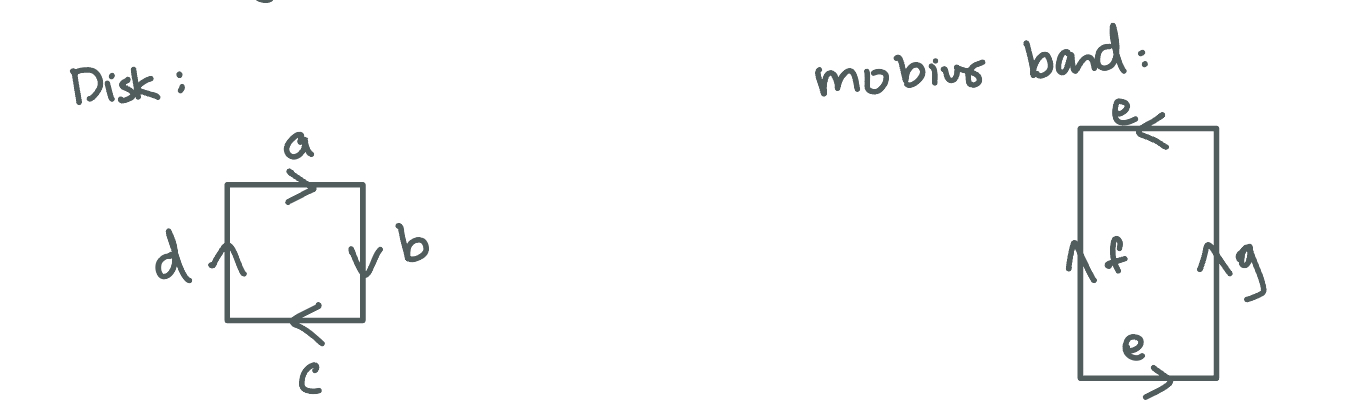
\includegraphics[width=0.7\linewidth]{1-1.jpeg} 
\end{figure}

Then, we glue $c$ and $b$ on the disk to $f$ on the Möbius band, which gives us the following:

\begin{figure}[h!] 
    \centering
    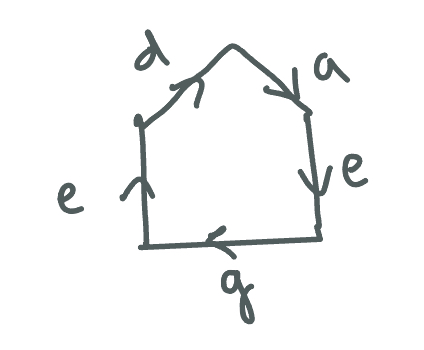
\includegraphics[width=0.3\linewidth]{1-2.jpeg} 
\end{figure}

Finally, we glue $d$ and $a$ to $g$.  


\begin{figure}[H] 
    \centering
    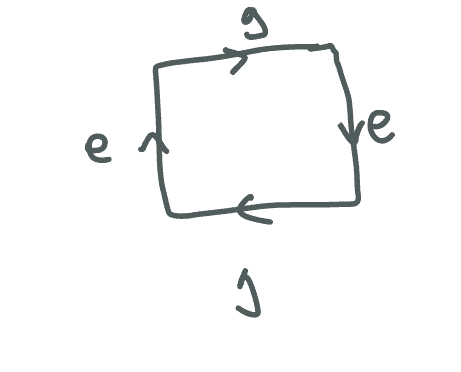
\includegraphics[width=0.3\linewidth]{1-3.jpeg} 
\end{figure}

This is the projective plane, as desired.

% DONE
\newpage

\item We will demonstrate that the surface obtained if you attach two Möbius bands along the sphere with two holes is a Klein bottle.

We begin with our open sphere and our Möbius band.

\begin{figure}[h!] 
    \centering
    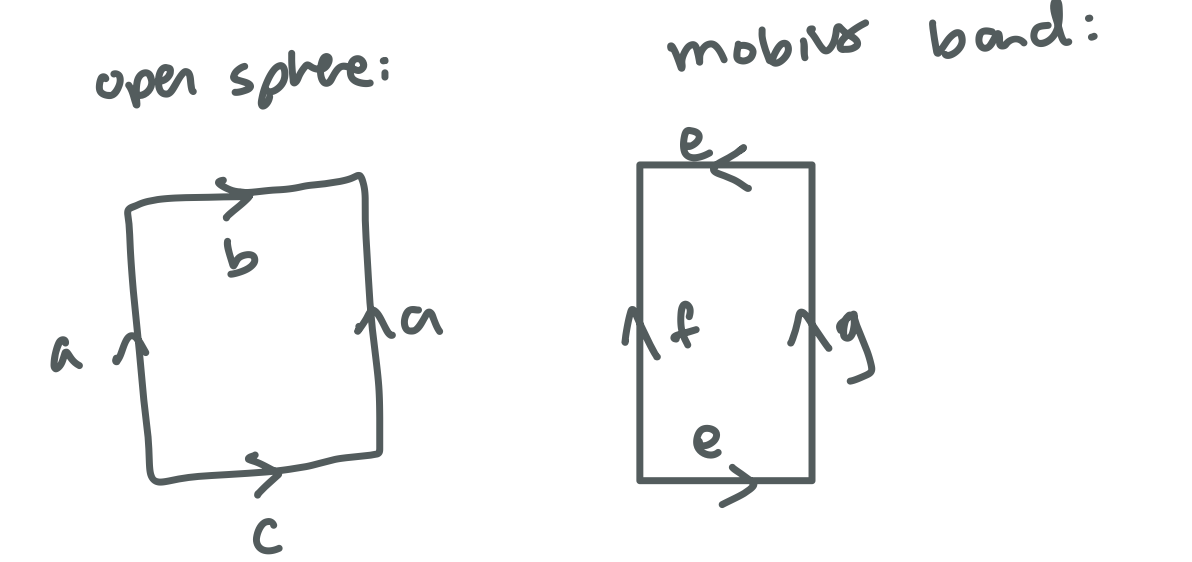
\includegraphics[width=0.7\linewidth]{2-1.png} 
\end{figure}

Then, rewrite the edges on the sphere as follows:
\begin{figure}[h!] 
    \centering
    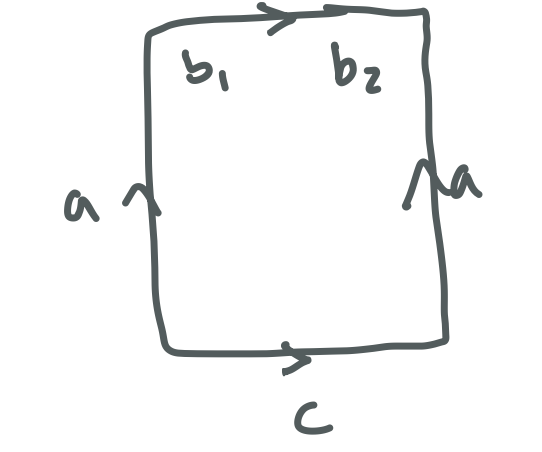
\includegraphics[width=0.3\linewidth]{2-2.png} 
\end{figure}

The, we glue $g$ to $b_1$:
\begin{figure}[H] 
    \centering
    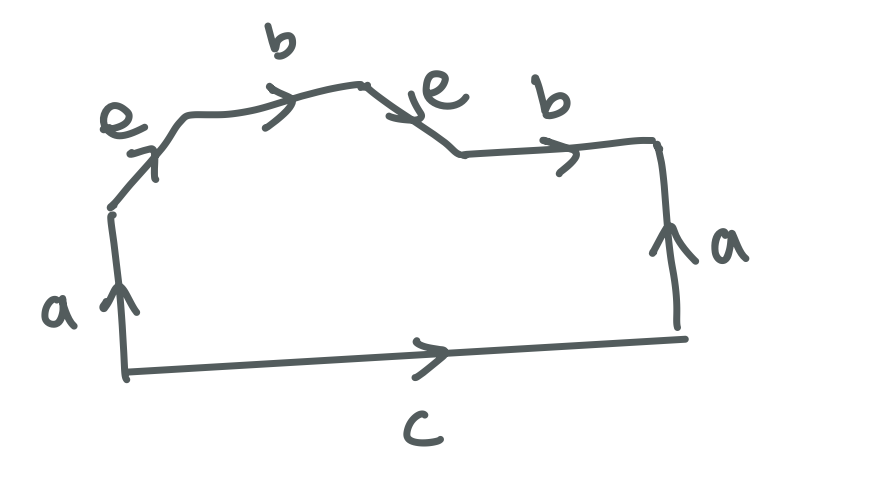
\includegraphics[width=0.5\linewidth]{2-3.png} 
\end{figure}

After that, we can combine the edges, where we use a new label, $g$ to represent $e$ and $b$.
\begin{figure}[H] 
    \centering
    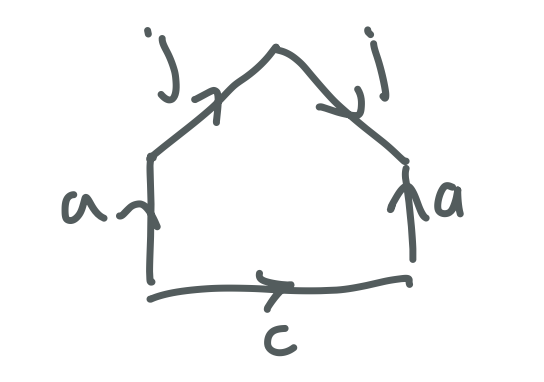
\includegraphics[width=0.3\linewidth]{2-4.png} 
\end{figure}

Apply the same logic we did for the "top" of the shape to the bottom, where we divide it into two segments and attach the mobius strip that way.

\begin{figure}[H] 
    \centering
    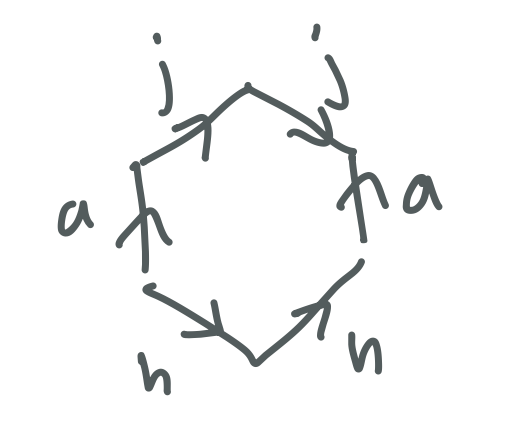
\includegraphics[width=0.3\linewidth]{2-5.png} 
\end{figure}

We can continously deform the shape where $a$ essentially becomes $0$ and it is still the same shape, so we can rewrite it. 

\begin{figure}[H] 
    \centering
    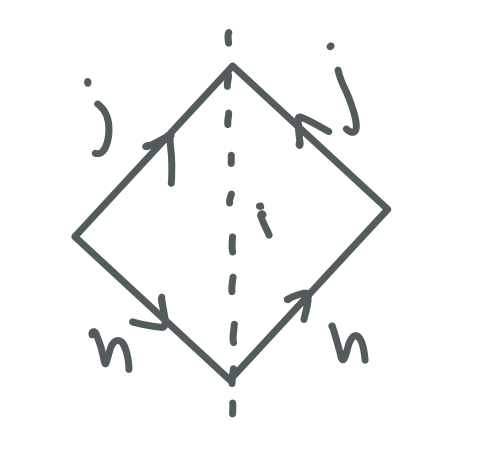
\includegraphics[width=0.3\linewidth]{2-6.png} 
\end{figure}

Then, we cut it in half and glue $j$ together, which gives us the following.

\begin{figure}[H] 
    \centering
    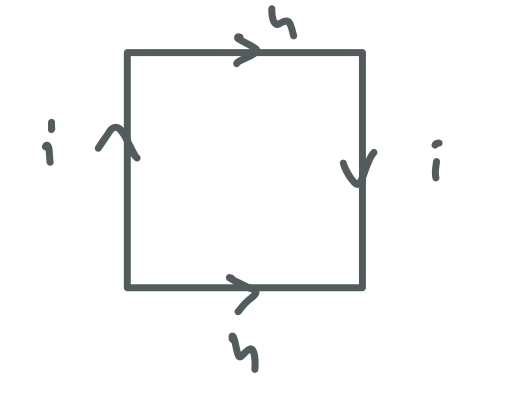
\includegraphics[width=0.3\linewidth]{2-7.png} 
\end{figure}

This is the Klein bottle, as desired.

\newpage
\item 
We will determine that the surface obtained by attaching a Möbius band along the boundary of a torus with a hole. 

First, we will begin by proving a lemma that will aide in the proof later. Begin with a mobius strip and Klein bottle.

\begin{figure}[H] 
    \centering
    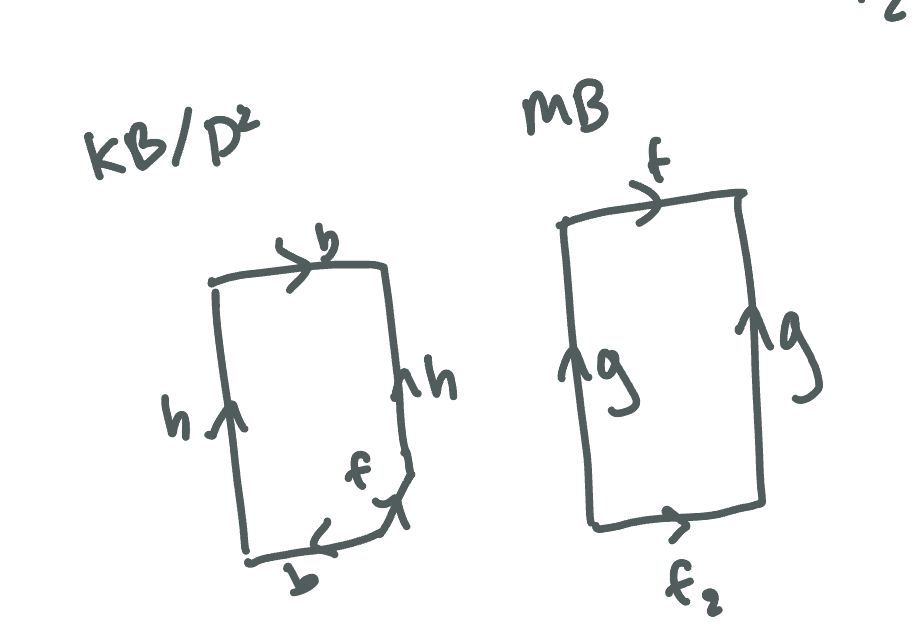
\includegraphics[width=0.4\linewidth]{3l-1.jpeg} 
\end{figure}

Glue them together along the boundary of the Klein bottle.


% \begin{figure}[H] 
%     \centering
%     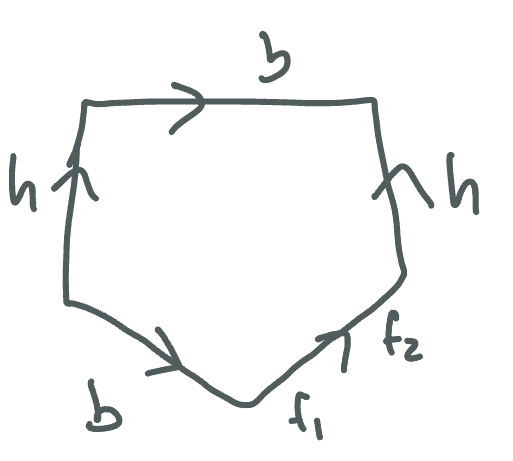
\includegraphics[width=0.3\linewidth]{3l-2.jpeg} 
% \end{figure}

This gives us the following shape when we are done gluing the Möbius band to the Klein bottle: 

\begin{figure}[H] 
    \centering
    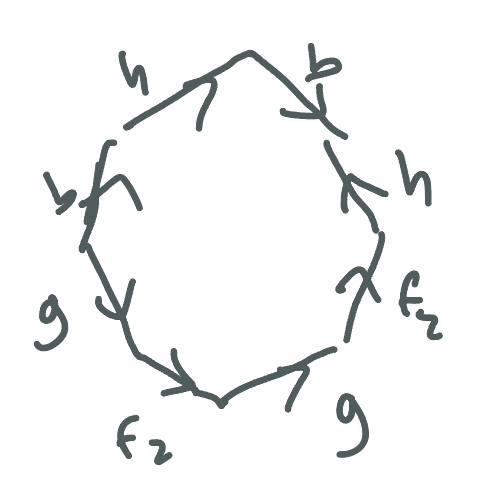
\includegraphics[width=0.3\linewidth]{3l-3.jpeg} 
\end{figure}

Then, we can cut the shape as follows to reglue it.

\begin{figure}[H] 
    \centering
    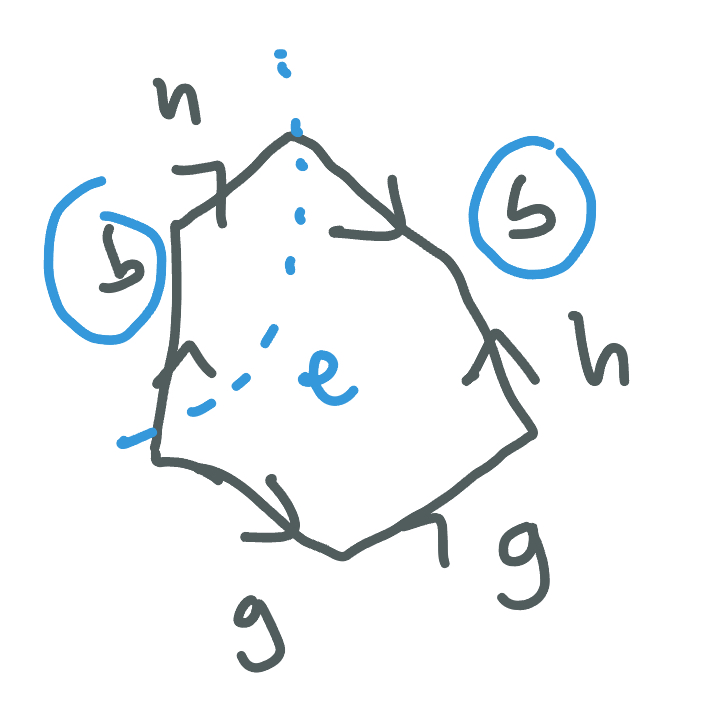
\includegraphics[width=0.3\linewidth]{3l-4.jpeg} 
\end{figure}

\begin{figure}[H] 
    \centering
    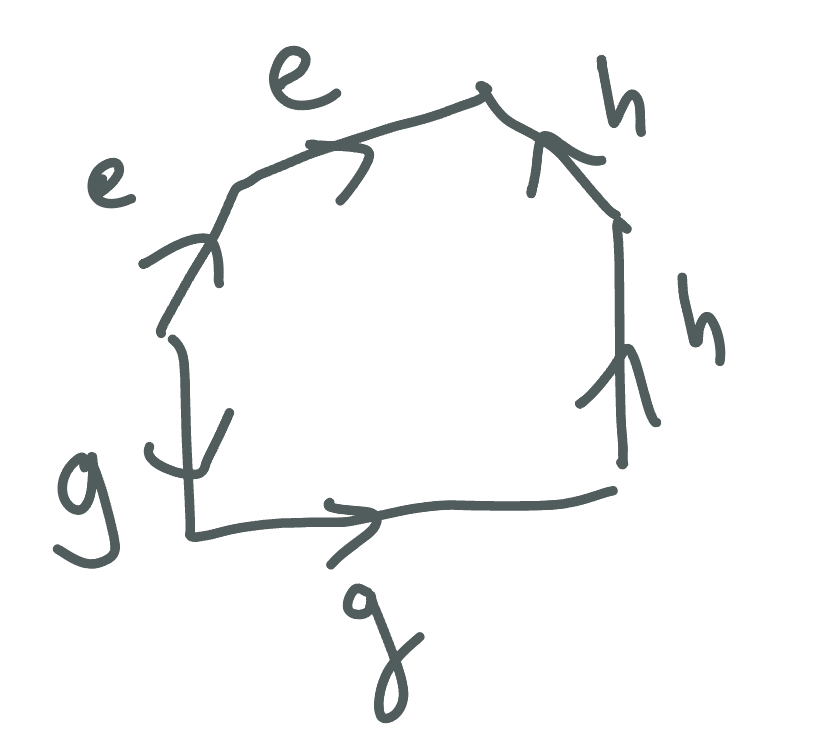
\includegraphics[width=0.3\linewidth]{3l-5.jpeg} 
\end{figure}

Let that be our result of the lemma for now. 

Returning to the initial problem, we begin with our torus with a hole and our Möbius band.

\begin{figure}[H] 
    \centering
    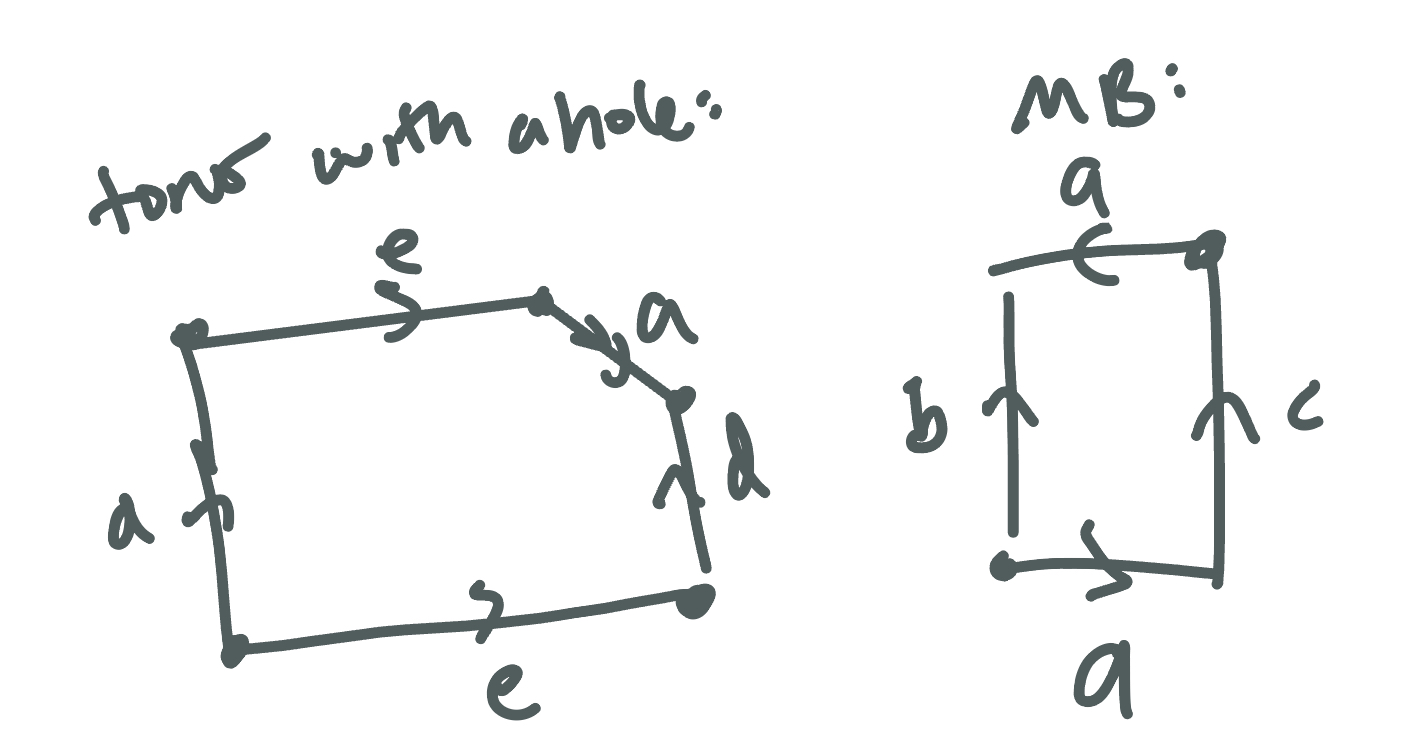
\includegraphics[width=0.5\linewidth]{3-1.jpeg} 
\end{figure}

Begin by cutting the Möbius band in half. 

\begin{figure}[H] 
    \centering
    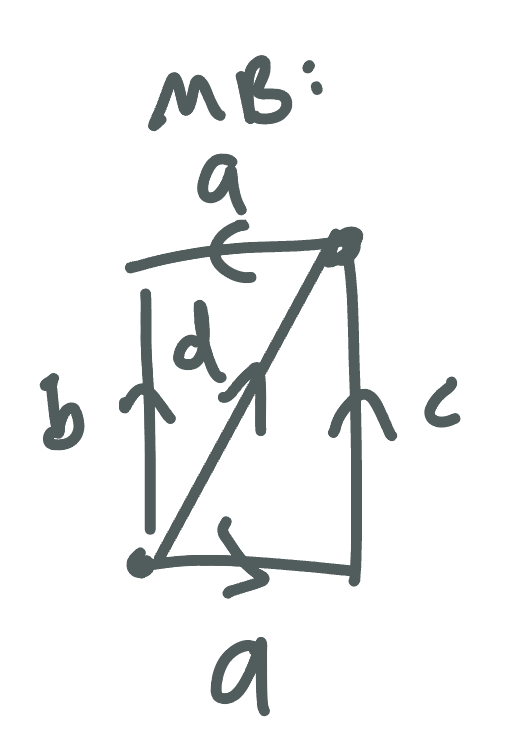
\includegraphics[width=0.2\linewidth]{3-2.jpeg} 
\end{figure}

Then, glue the Möbius band along a, creating the following shape.
\begin{figure}[H] 
    \centering
    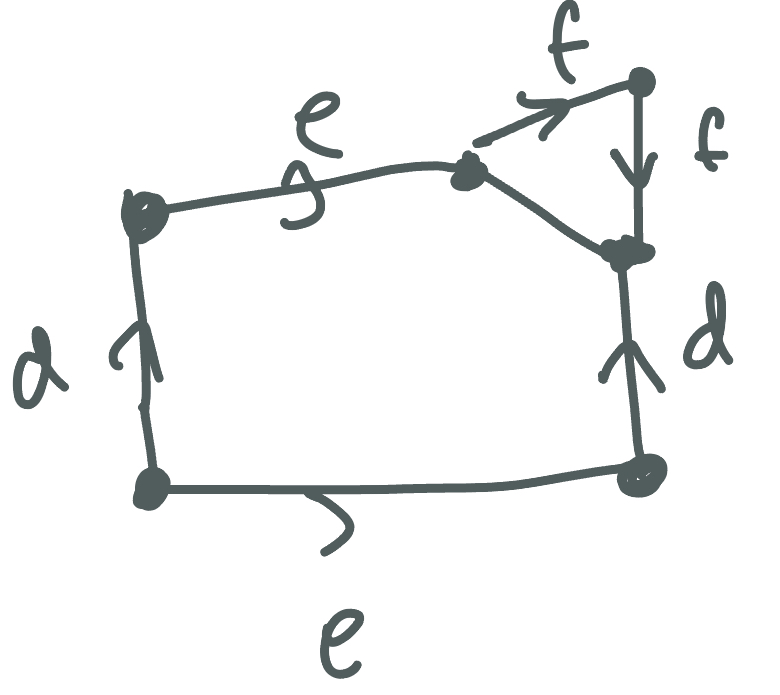
\includegraphics[width=0.3\linewidth]{3-3.jpeg} 
\end{figure}

The, we can add a new cut, along $g$, which gives us the following:

\begin{figure}[H] 
    \centering
    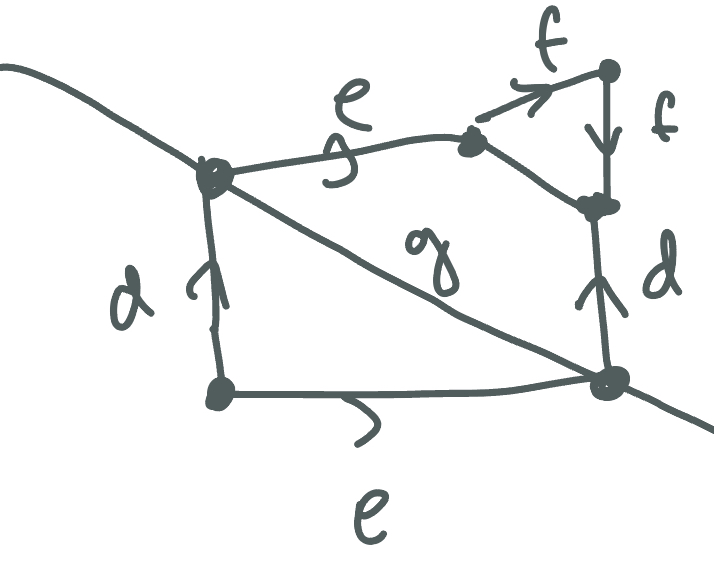
\includegraphics[width=0.3\linewidth]{3-4.jpeg} 
\end{figure}

Now, we can glue across $e$, which gives the following: 

\begin{figure}[H] 
    \centering
    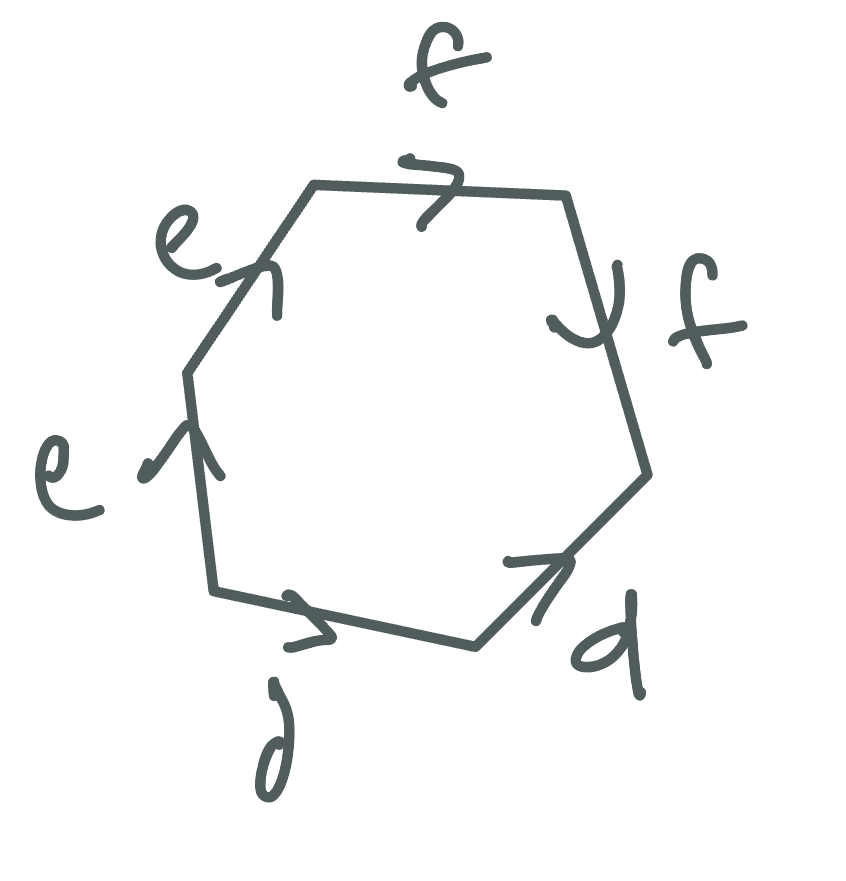
\includegraphics[width=0.3\linewidth]{3-5.jpeg} 
\end{figure}


This is clearly homeomorphic to the shape we proved in our lemma, meaning the shape we are currently at is equivalent to a Möbius band and a Klein bottle. 

Three projective planes are topologically equivalent to a Möbius band and a Klein bottle. That is also topologically equivalent to a Klein bottle and a projective plane, since $KB \cong P^2 \# P^2$. Thus, through proving this homeomorphism with the lemma, we have overall proved that hte surface is the connected sum of the Klein bottle and the projective plane. 


% TODO: maybe add something about the disk / figure out tf is going on 


\newpage
\item Now, we will compute the genus of the following 5 surfaces. The mathematical definition of genus that we will be using to compute these values is as follows: the maximum number of non intersecting circular cuts that can be made without disconnecting the space.

For the remainder of the problems, we will be referring to the surfaces using the numbers that are indicated in the following diagram: 


\begin{figure}[H] 
    \centering
    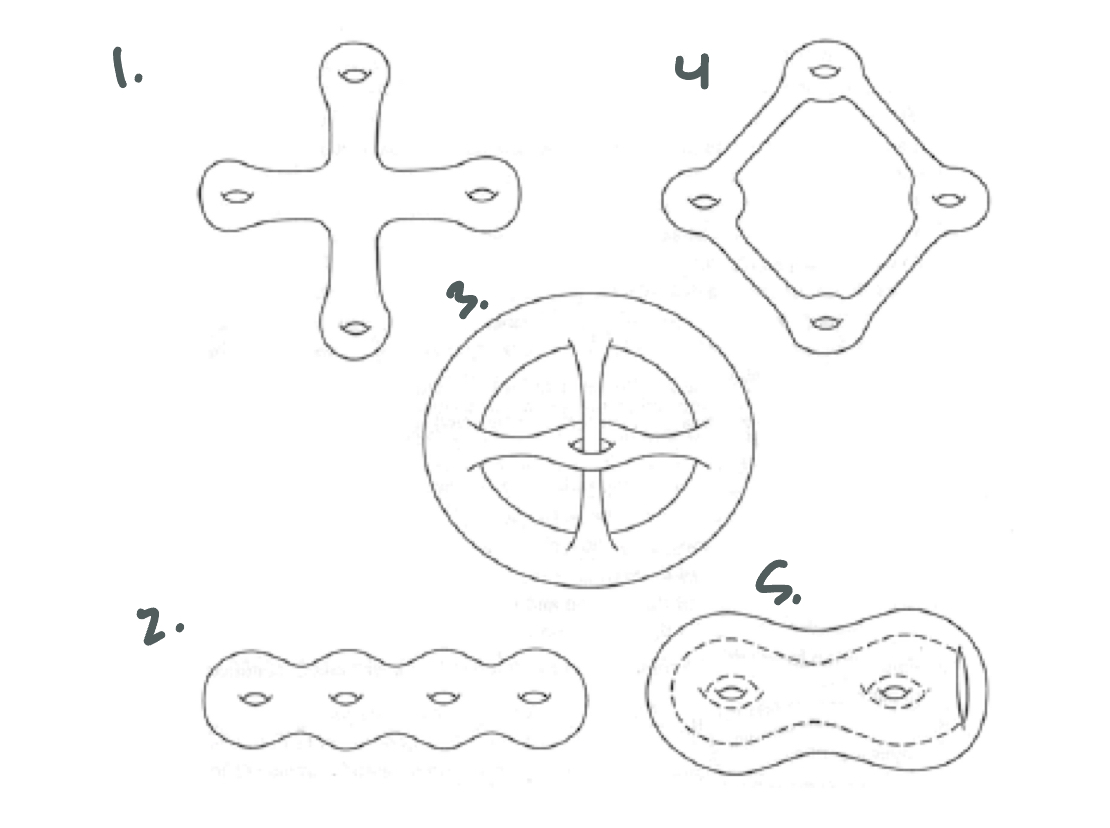
\includegraphics[width=0.5\linewidth]{4-1.jpeg} 
\end{figure}

For surfaces 1-4, calculating the genus is straightforward as it can clearly be done visually. THe genuses are as follows: surface 1 has genus 4, surface 2 has genus 4, surface 3 has genus 4, and surface 4 has genus 5. There are of course, multiple sets of cuts that can work, but to demonstrate the solution, the following cuts can be made: 


\begin{figure}[H] 
    \centering
    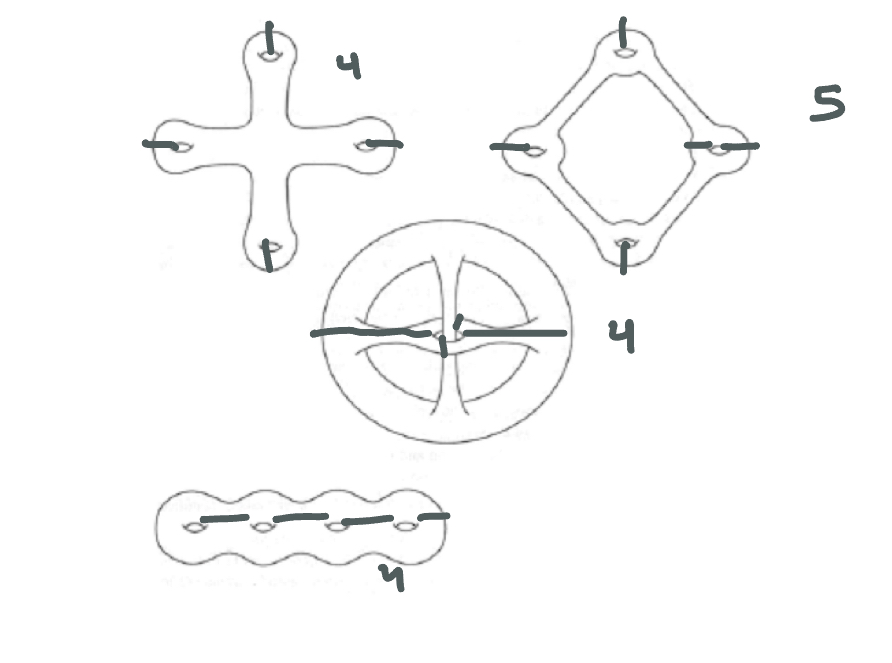
\includegraphics[width=0.5\linewidth]{4-2.jpeg} 
\end{figure}

Now, we will deal with surface 5. Imagine a continous deformation of surface 5, where we are opening it up utilizing the hole on the side. If we stretch it out far enough, we can clearly see that each segment turns into two clear holes, where the holes alternate in direction. 


\begin{figure}[H] 
    \centering
    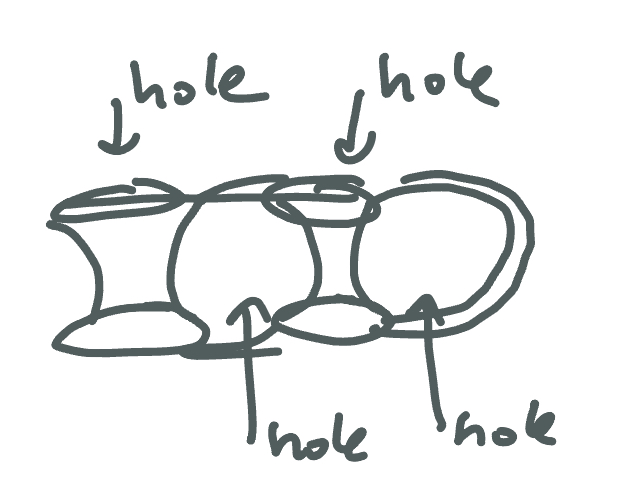
\includegraphics[width=0.3\linewidth]{4-3.jpeg} 
\end{figure}

Now that we have reduced this surface to a more simple problem, we can clearly find the genus of 4:


\begin{figure}[H] 
    \centering
    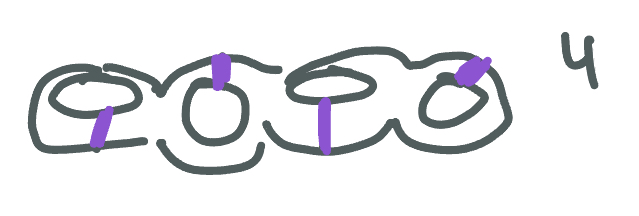
\includegraphics[width=0.3\linewidth]{4-4.jpeg} 
\end{figure}

\newpage
\item Now, we will look at the surfaces from the previous problem and determine which are homeomorphic.

Surface 4 cannot be homeomorphic with any of the other surfaces since it has a different genus, which is a topological invariant. 

Surface 5 cannot be homeomorphic with any of the other surfaces since it has a different dimension, which is also a topological invariant. 

Thus, it is only possible for surfaces 1, 2, and/or 3 to be homeomorphic with each other. 

Clearly 1 and 2 are homeomorphic as we can create a continuous deformation between them as follows, which indicates a homeomorphism.
\begin{figure}[H] 
    \centering
    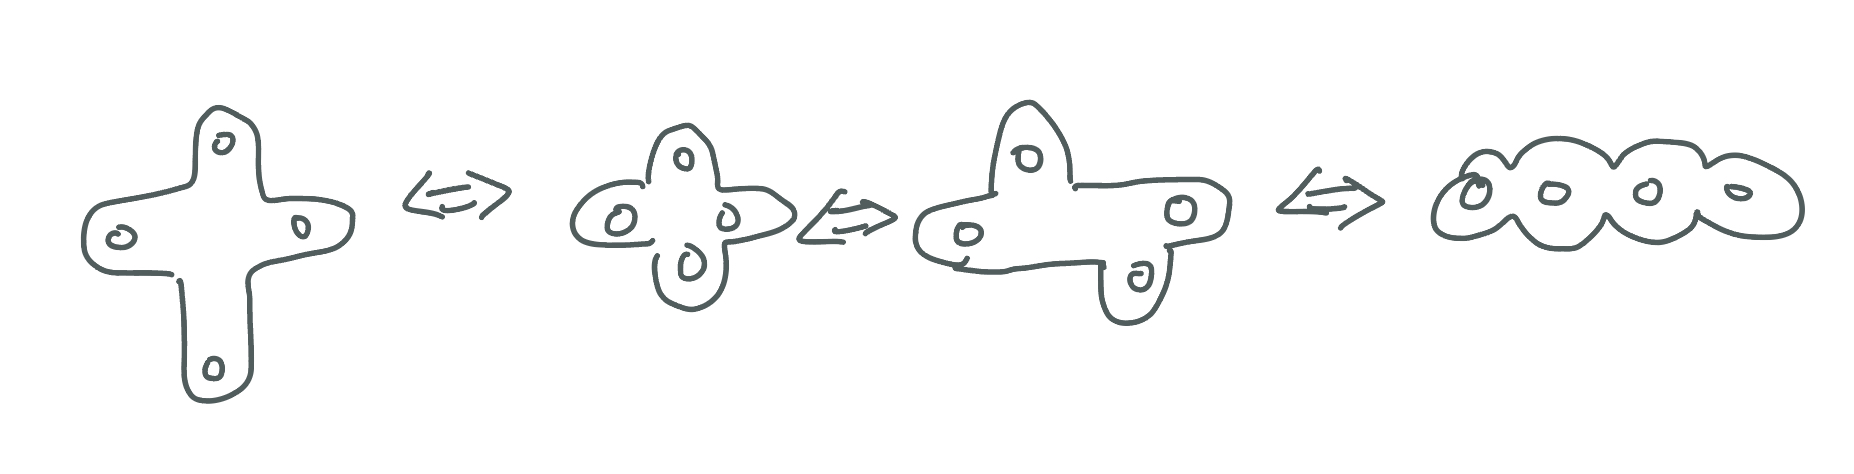
\includegraphics[width=0.5\linewidth]{5-1.jpeg} 
\end{figure}

However, 3 is not homeomorphic with them since it is impossible to create a continuous deformation as it is wrapping around itself in a way that cannot be "untangled," meaning that it doesn't align with 1 and 2.

Thus, only 1 and 2 are homeomorphic. 


\newpage
\item  Finally, we will compute the Euler characteristic of the genus one orientable surface with two boundary components via it's gluing diagram.

To compute the Euler characteristic of a surface like this, we will use the torus with two discs taken out of it, which should be topologically equivalent to any other surface that would meet the definition given.

The gluing diagram for this surface is as follows:

\begin{figure}[H] 
    \centering
    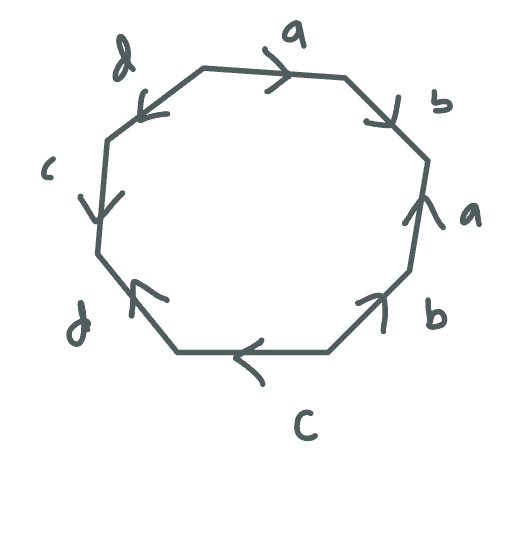
\includegraphics[width=0.3\linewidth]{6-1.jpeg} 
\end{figure}

Thus, we can use that in order to compute the Euler characteristic.

The Euler characteristic formula is as follows:

\[\chi (g) = V - E + F\]

Here, we can clearly see there is one face as well as 4 distinct edges (4 different letters used in the diagram). Finally, there are 3 vertices, as that represents the two boundary components as well as the shape itself. Thus, we can calculate:

\[= 3 - 4 + 1\]
\[=0\]


\end{enumerate}

\end{document}